\section{K-Armed-Bandits}
Before we look at algorithms for the case where we do not have a model of the 
world, we will talk about the k-armed-bandit problem, which helps us to understand decision 
making under uncertainty.\newline
A k-armed bandit is a tuple $(A,p(r|a))$, where $A$ is the known set of $k$ actions we can 
take (arm) and $p(r|a)$ is the unknown probability distribution over rewards. At each time 
step $t$ we take an action $a_t$ and the environment generates a reward $r_t$. The goal is 
to maximise the expected reward. To achieve this goal we have to decide which arm to pull, 
so we need to know the expected reward per action $\hat{q}$ (action value function)
$$ \hat{q}= \mathbb{E}[r_t|a_t=a] = \int p(r|a) r \;\texttt{d}r$$
Since we do not know $p(r|a)$, we approximate the integral by Monte Carlo simulation. 
$$\hat{q}= \mathbb{E}[r_t|a_t=a] \approx \frac{\sum_{i=1}^{t-1} \mathds{1}(a_i=a)r}
{\sum_{i=1}^{t-1} \mathds{1}(a_i=a)} = q_t(a)$$
Instead of storing all the rewards to calculate the sum, one can also reformulate 
it using an incremental update rule.
\begin{align*}
    q_{n+1} = \frac{1}{n}\sum_{i=1}^n r_i &= \frac{1}{n} \left(r_n+ \sum_{i=1}^{n-1} r_i \right) \\
    &= \frac{1}{n} \left(r_n+ (n-1){\color{blue}\frac{1}{n-1}\sum_{i=1}^{n-1} r_i} \right) \\
    &=  \frac{1}{n} \left(r_n+ (n-1){\color{blue}q_n} \right)\\
    &= q_n + \frac{1}{n}(r_n-q_n) \numberthis \label{eq:running_avg}
\end{align*}
This formulation is called the sampled average method, whereas the more general update rule looks like this.
$$q_{n+1} = q_n + \alpha_n (r_n-q_n)$$
We will now consider different strategies for choosing actions to maximise the expected 
reward.
\subsection{Greedy action selection}
In greedy action selection, our next action $a_t$ is defined as $$a_t = \argmax\limits_{a\in 
A} q_t(a)$$ The problem with this approach is that we could get stuck in a suboptimal 
policy. Consider the following example where we have three actions $a_1,a_2,a_3$ to choose 
from with unknown true rewards ${q(a_1)=0.95,q(a_2)=0.9,q(a_3)=0.1}$. We know have as the 
initial q-values the values \newline ${q(a_1)= q(a_3) = 0,q(a_2)=1}$. From there on we do 
greedy action selection, which results in only picking the action $a_2$ even though the 
actual best action to take is $a_1$, but for that we would have to drift from our strategy. 
This is the core problem in RL. We need to make a trade-off between Exploration: Improve 
knowledge for long term benefit and Exploitation: Using knowledge for short-term benefit. 
One way to achieve this is called $\epsilon$-greedy exploration, 
where we choose a value $\epsilon \in [0,1]$ representing the probability of 
exploring/exploiting.
$$ a = \left\{
\begin{array}{ll}
\argmax_a q_t(a) & \text{with probability } 1-\epsilon \\
\text{Uniform}({a_1,\dots,a_k}) & \, \text{with probability } \epsilon\\
\end{array}
\right.$$

\subsection{Exploration and Entropy}
Although $\epsilon$ greedy action selection is an effective means of balancing exploration 
and exploitation in reinforcement learning, one 
drawback is that when it explores, it chooses equally among all actions. 
This means that it is just as likely to choose the worst appearing 
action as it does the next best action. In tasks where the worst actions are very bad, this 
can be unsatisfactory. The obvious solution is to vary the action probabilities as a  
graded function of the estimated value (exploitation). But at the same time, we are 
uncertain about the rewards and therefore need to keep uncertainty in the policy, for which 
entropy is a good measure (exploration). Thus the objective looks like this 
\begin{align*}
    \pi^*_t = \argmax\limits_\pi \sum_a \pi(a) q_t(a) + \tau^{-1}H(\pi) &=\argmax\limits_\pi \sum_a \pi(a) q_t(a) + \tau^{-1} (- \sum_a \pi(a)\log{\pi(a)})\\   &=\argmax\limits_\pi \sum_a \pi(a)(q_t(a)-\tau^{-1}\log{\pi(a)})
\end{align*}
Calculation the derivative and setting it equal to zero gives us the policy which maximises the objective $$ \pi(a)= \frac{\exp(\tau q_t(a))}{\sum_{a'}\exp(\tau q_t(a'))}$$

\subsection{Optimistic Value Initialization}
The idea is simply to initialise the q-values with optimistic values, this has the effect of 
adding a positive bias to less explored actions, thus forcing exploration.

\subsection{Upper-Confidence-Bounds (UCB)}\label{UCB}
The UCB formula is defined as $$ a_t = \argmax\limits_a 
\underbrace{q_t(a)}_{\text{exploitation}} + \underbrace{c \sqrt{\frac{\log{t}}
{N_t(a)}}}_{\text{exploration}}$$
$c$ is a constant that allows us to set the exploration/exploitation trade-off. 
$\sqrt{1/{N_t(a)}}$ essentially says that the more times you pull an arm, there is less unknown about that arm. 
So the fewer times action a is chosen, the higher the exploration bonus.
$\sqrt{\log{t}}$ ensures that you don't stop exploring too early. \newline 
In the following, we will examine how different strategies perform across various parameter settings. 
To do this, we utilize a 10-armed bandit experiment, averaging the results over 2000 runs with sample 
average action-value estimates.

\begin{figure}[H]
    \centering
    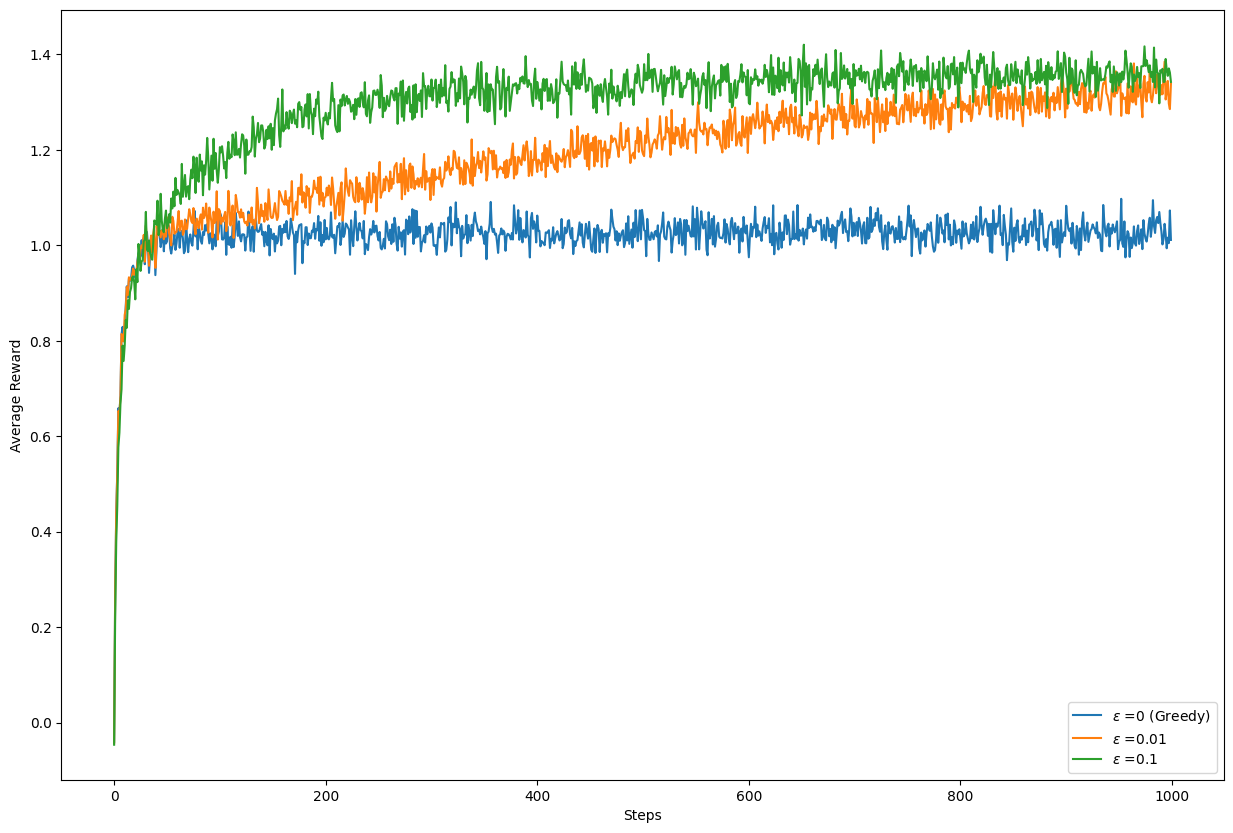
\includegraphics[width=\linewidth, height=0.33\textheight]{images/bandit_greedy.png}
    \caption{$\epsilon$-Greedy}
\end{figure}

\begin{figure}[H]
\vspace{-1.5cm}
    \centering
   \begin{minipage}{\linewidth}
        \centering
        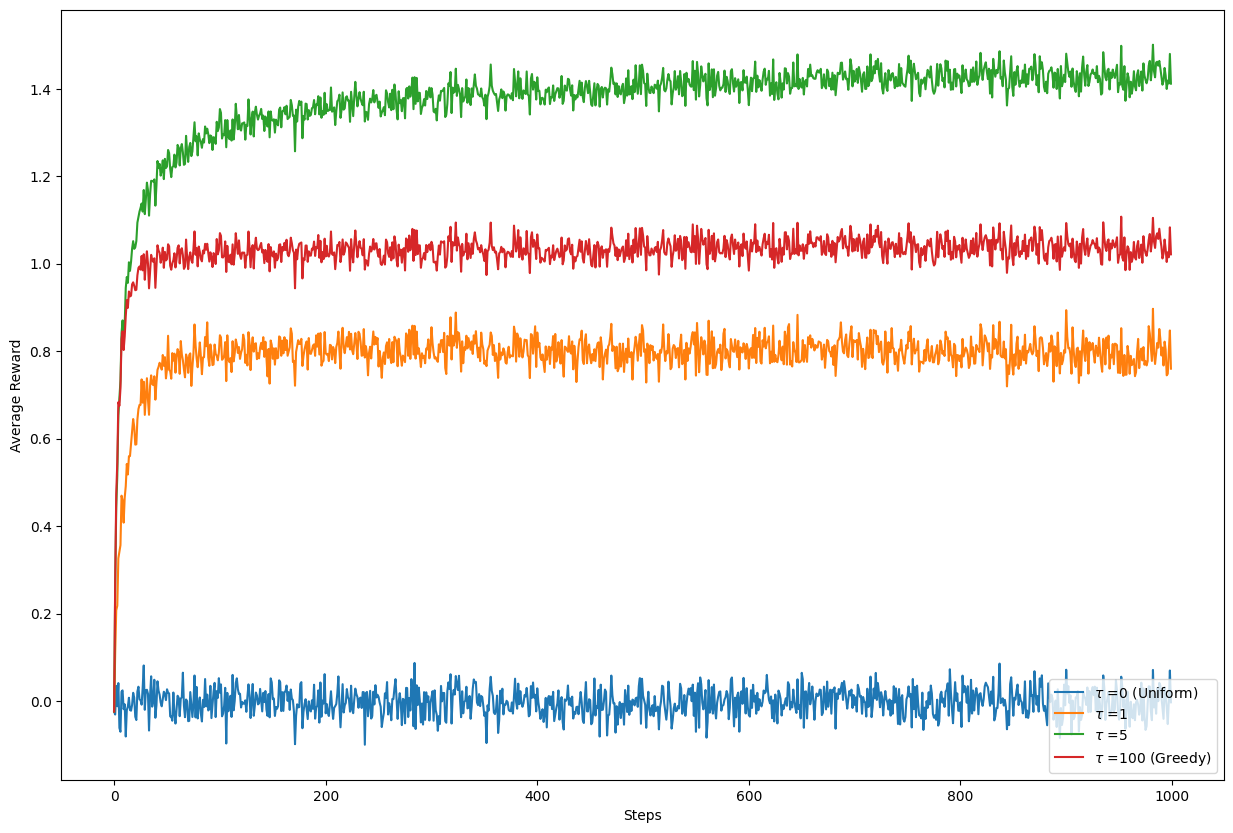
\includegraphics[width=\linewidth, height=0.33\textheight]{images/bandit_softmax.png}
        \caption{Softmax}
    \end{minipage}
    
    
    \vspace{0.5mm} % Small spacing between minipages
    
     \begin{minipage}{\linewidth}
        \centering
        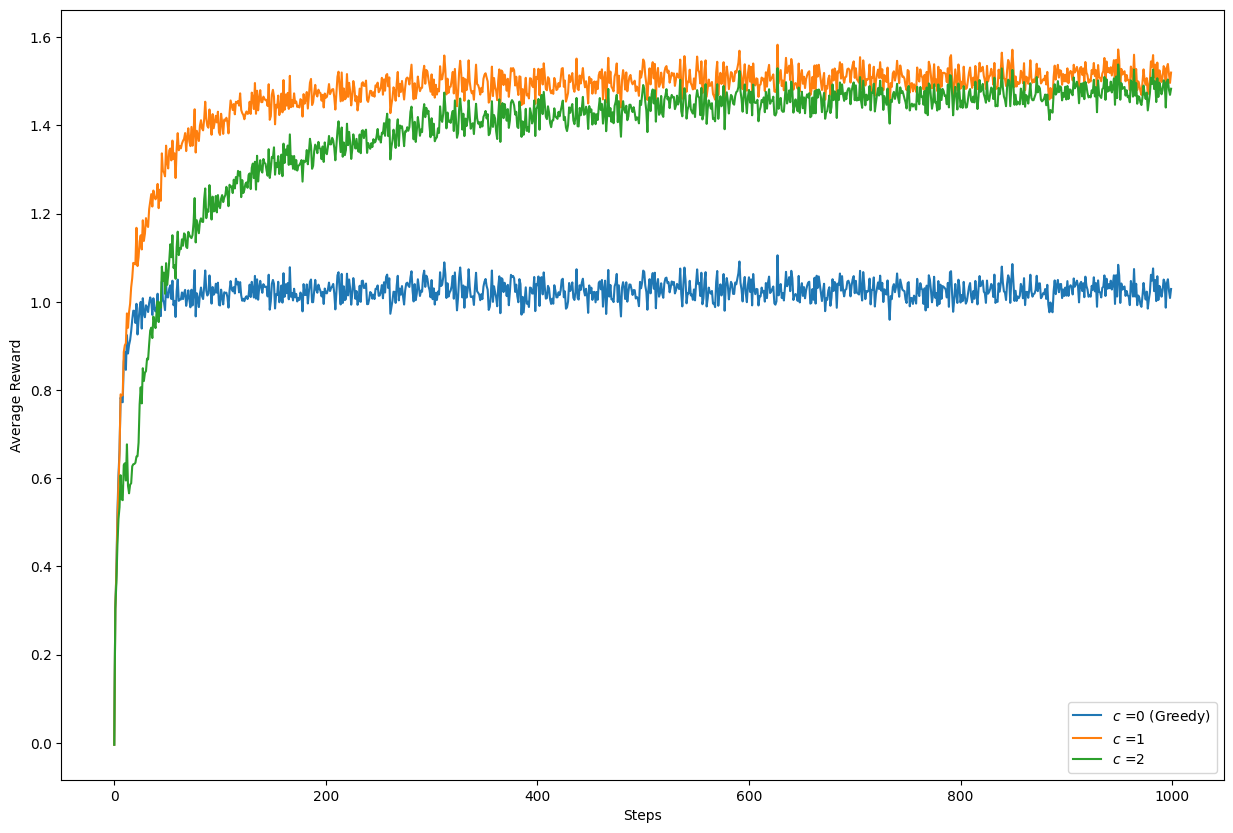
\includegraphics[width=\linewidth, height=0.33\textheight]{images/bandit_ucb.png}
        \caption{UCB}
    \end{minipage}
    
    
    \vspace{0.5mm}
    
    \begin{minipage}{\linewidth}
        \centering
     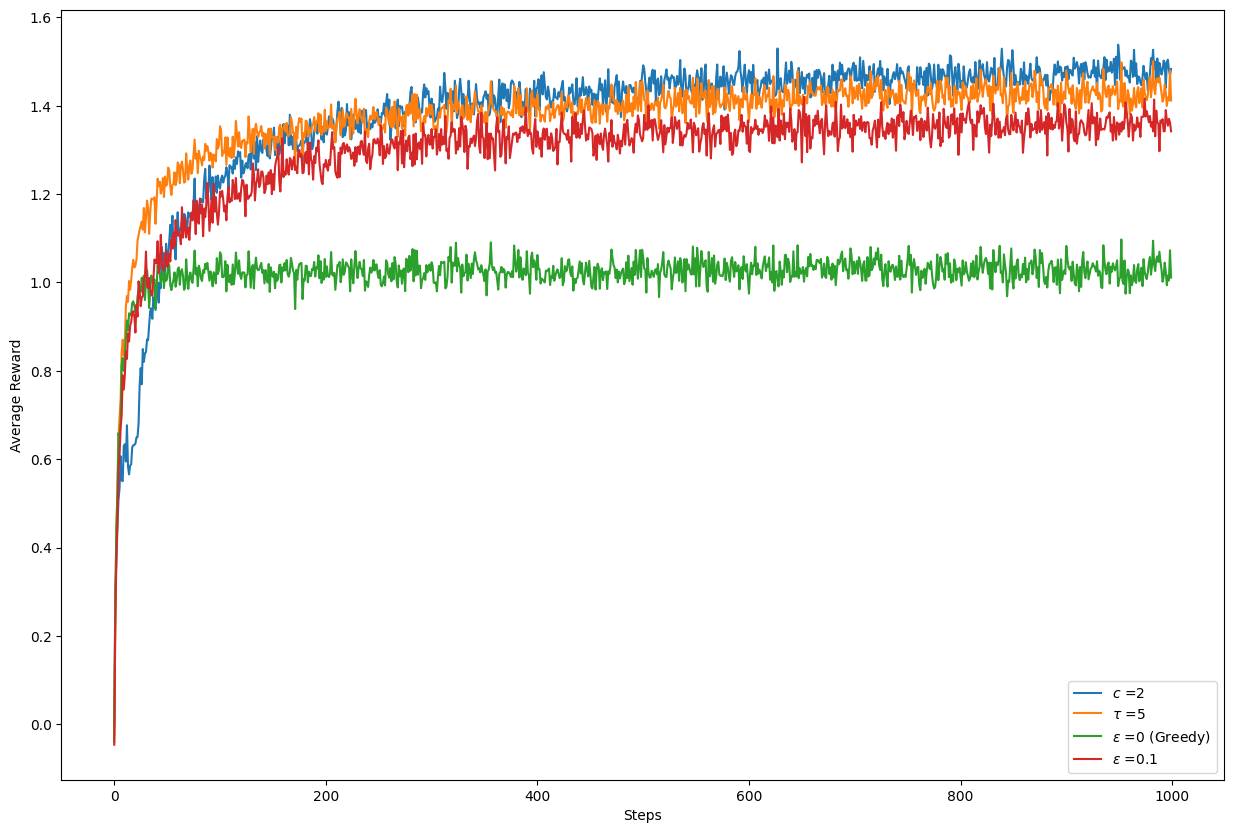
\includegraphics[width=\linewidth, height=0.33\textheight]{images/bandit_comparison.png}
    \caption{Comparison of different strategies}
    \end{minipage}
    
    \label{fig:three-methods}
\end{figure}